\documentclass[symmetric,justified,marginals=raggedouter]{tufte-book}

%\hypersetup{colorlinks}% uncomment this line if you prefer colored hyperlinks (e.g., for onscreen viewing)

%%
% If they're installed, use Bergamo and Chantilly from www.fontsite.com.
% They're clones of Bembo and Gill Sans, respectively.
%\IfFileExists{bergamo.sty}{\usepackage[osf]{bergamo}}{}% Bembo
%\IfFileExists{chantill.sty}{\usepackage{chantill}}{}% Gill Sans

%\usepackage{microtype}

%%
% For nicely typeset tabular material
\usepackage{booktabs}

%%
% For graphics / images
\usepackage{graphicx}
\setkeys{Gin}{width=\linewidth,totalheight=\textheight,keepaspectratio}
\graphicspath{{graphics/}}

% The fancyvrb package lets us customize the formatting of verbatim
% environments.  We use a slightly smaller font.
\usepackage{fancyvrb}
\fvset{fontsize=\normalsize}

%%
% Prints argument within hanging parentheses (i.e., parentheses that take
% up no horizontal space).  Useful in tabular environments.
\newcommand{\hangp}[1]{\makebox[0pt][r]{(}#1\makebox[0pt][l]{)}}

%%
% Prints an asterisk that takes up no horizontal space.
% Useful in tabular environments.
\newcommand{\hangstar}{\makebox[0pt][l]{*}}

%%
% Prints a trailing space in a smart way.
\usepackage{xspace}

%%
% Some shortcuts for Tufte's book titles.  The lowercase commands will
% produce the initials of the book title in italics.  The all-caps commands
% will print out the full title of the book in italics.
\newcommand{\vdqi}{\textit{VDQI}\xspace}
\newcommand{\ei}{\textit{EI}\xspace}
\newcommand{\ve}{\textit{VE}\xspace}
\newcommand{\be}{\textit{BE}\xspace}
\newcommand{\VDQI}{\textit{The Visual Display of Quantitative Information}\xspace}
\newcommand{\EI}{\textit{Envisioning Information}\xspace}
\newcommand{\VE}{\textit{Visual Explanations}\xspace}
\newcommand{\BE}{\textit{Beautiful Evidence}\xspace}

\newcommand{\TL}{Tufte-\LaTeX\xspace}

% Prints the month name (e.g., January) and the year (e.g., 2008)
\newcommand{\monthyear}{%
  \ifcase\month\or January\or February\or March\or April\or May\or June\or
  July\or August\or September\or October\or November\or
  December\fi\space\number\year
}


% Prints an epigraph and speaker in sans serif, all-caps type.
\newcommand{\openepigraph}[2]{%
  %\sffamily\fontsize{14}{16}\selectfont
  \begin{fullwidth}
  \sffamily\large
  \begin{doublespace}
  \noindent\allcaps{#1}\\% epigraph
  \noindent\allcaps{#2}% author
  \end{doublespace}
  \end{fullwidth}
}

% Inserts a blank page
\newcommand{\blankpage}{\newpage\hbox{}\thispagestyle{empty}\newpage}

\usepackage{units}

% Typesets the font size, leading, and measure in the form of 10/12x26 pc.
\newcommand{\measure}[3]{#1/#2$\times$\unit[#3]{pc}}

% Macros for typesetting the documentation
\newcommand{\hlred}[1]{\textcolor{Maroon}{#1}}% prints in red
\newcommand{\hangleft}[1]{\makebox[0pt][r]{#1}}
\newcommand{\hairsp}{\hspace{1pt}}% hair space
\newcommand{\hquad}{\hskip0.5em\relax}% half quad space
\newcommand{\TODO}{\textcolor{red}{\bf TODO!}\xspace}
\newcommand{\ie}{\textit{i.\hairsp{}e.}\xspace}
\newcommand{\eg}{\textit{e.\hairsp{}g.}\xspace}
\newcommand{\na}{\quad--}% used in tables for N/A cells
\providecommand{\XeLaTeX}{X\lower.5ex\hbox{\kern-0.15em\reflectbox{E}}\kern-0.1em\LaTeX}
\newcommand{\tXeLaTeX}{\XeLaTeX\index{XeLaTeX@\protect\XeLaTeX}}
% \index{\texttt{\textbackslash xyz}@\hangleft{\texttt{\textbackslash}}\texttt{xyz}}
\newcommand{\tuftebs}{\symbol{'134}}% a backslash in tt type in OT1/T1
\newcommand{\doccmdnoindex}[2][]{\texttt{\tuftebs#2}}% command name -- adds backslash automatically (and doesn't add cmd to the index)
\newcommand{\doccmddef}[2][]{%
  \hlred{\texttt{\tuftebs#2}}\label{cmd:#2}%
  \ifthenelse{\isempty{#1}}%
    {% add the command to the index
      \index{#2 command@\protect\hangleft{\texttt{\tuftebs}}\texttt{#2}}% command name
    }%
    {% add the command and package to the index
      \index{#2 command@\protect\hangleft{\texttt{\tuftebs}}\texttt{#2} (\texttt{#1} package)}% command name
      \index{#1 package@\texttt{#1} package}\index{packages!#1@\texttt{#1}}% package name
    }%
}% command name -- adds backslash automatically
\newcommand{\doccmd}[2][]{%
  \texttt{\tuftebs#2}%
  \ifthenelse{\isempty{#1}}%
    {% add the command to the index
      \index{#2 command@\protect\hangleft{\texttt{\tuftebs}}\texttt{#2}}% command name
    }%
    {% add the command and package to the index
      \index{#2 command@\protect\hangleft{\texttt{\tuftebs}}\texttt{#2} (\texttt{#1} package)}% command name
      \index{#1 package@\texttt{#1} package}\index{packages!#1@\texttt{#1}}% package name
    }%
}% command name -- adds backslash automatically
\newcommand{\docopt}[1]{\ensuremath{\langle}\textrm{\textit{#1}}\ensuremath{\rangle}}% optional command argument
\newcommand{\docarg}[1]{\textrm{\textit{#1}}}% (required) command argument
\newenvironment{docspec}{\begin{quotation}\ttfamily\parskip0pt\parindent0pt\ignorespaces}{\end{quotation}}% command specification environment
\newcommand{\docenv}[1]{\texttt{#1}\index{#1 environment@\texttt{#1} environment}\index{environments!#1@\texttt{#1}}}% environment name
\newcommand{\docenvdef}[1]{\hlred{\texttt{#1}}\label{env:#1}\index{#1 environment@\texttt{#1} environment}\index{environments!#1@\texttt{#1}}}% environment name
\newcommand{\docpkg}[1]{\texttt{#1}\index{#1 package@\texttt{#1} package}\index{packages!#1@\texttt{#1}}}% package name
\newcommand{\doccls}[1]{\texttt{#1}}% document class name
\newcommand{\docclsopt}[1]{\texttt{#1}\index{#1 class option@\texttt{#1} class option}\index{class options!#1@\texttt{#1}}}% document class option name
\newcommand{\docclsoptdef}[1]{\hlred{\texttt{#1}}\label{clsopt:#1}\index{#1 class option@\texttt{#1} class option}\index{class options!#1@\texttt{#1}}}% document class option name defined
\newcommand{\docmsg}[2]{\bigskip\begin{fullwidth}\noindent\ttfamily#1\end{fullwidth}\medskip\par\noindent#2}
\newcommand{\docfilehook}[2]{\texttt{#1}\index{file hooks!#2}\index{#1@\texttt{#1}}}
\newcommand{\doccounter}[1]{\texttt{#1}\index{#1 counter@\texttt{#1} counter}}

% Generates the index
\usepackage{makeidx}
\makeindex


\usepackage{indentfirst}

\usepackage[utf8]{inputenc}
\usepackage[T1]{fontenc}

%%%%%%%%%%%%%%%%%%%%%%%%%%%%%%%% Customization %%%%%%%%%%%%%%%%%%%%%%%%%%%%%%%%

\setcounter{tocdepth}{1}
\setcounter{secnumdepth}{1}

\renewcommand\contentsname{\normalfont \huge Table des matières}

\titlecontents{chapter}%
    [0em]% distance from left margin
    {\vspace{1\baselineskip}\begin{fullwidth}Chapitre }% above (global formatting of entry)
    {\contentslabel{0em} \hspace{1em} \huge $\vert$ \Large}% before w/ label (label = ``Chapter 1'')
    {\hspace{1em}}% before w/o label
    {\hfill\qquad\thecontentspage}% filler and page (leaders and page num)
    [\end{fullwidth}]% after
\titlecontents{section}% FIXME
    [0em] % distance from left margin
    {\vspace{0\baselineskip}\begin{fullwidth} \rmfamily\itshape} % above (global formatting of entry)
    {\hspace*{6em}\contentslabel{2em}} % before w/label (label = ``2.6'')
    {\hspace*{7em}} % before w/o label
    {\normalfont\hfill\qquad\thecontentspage} % filler + page (leaders and page num)
    [\end{fullwidth}] % after

\usepackage{enumitem}
\setlist{leftmargin=10mm}

\begin{document}

% Front matter
\frontmatter

%%%%%%%%%%%%%%%%%%%%%%%%%%%%%%%%%%%% Titre %%%%%%%%%%%%%%%%%%%%%%%%%%%%%%%%%%%%

\newpage
\author{Quentin Lobbé}
\title{\nohyphenation{Archives et Fragments Web}}
\cleardoublepage
{  
  \begin{fullwidth}%
  \thispagestyle{empty} 
  \setlength{\parskip}{\baselineskip}
  \begingroup
  \vspace*{10em}
  \par\noindent\Large{Quentin Lobbé}
  \vspace*{-1em}
  \par\noindent\Huge\textbf{Archives et Fragments Web}
  \par\noindent\nohyphenation\Large{Désagréger les archives Web pour mener une exploration temporelle de traces numériques des migrations}
  \endgroup
  \vfill  
  \par\noindent\nohyphenation Université Paris-Saclay, École doctorale des sciences et technologies de l'information et de la communication.  Thèse pour l'obtention du doctorat de Télécom ParisTech et de l'Université Paris-Saclay.    
  \end{fullwidth}%
}

\blankpage

%%%%%%%%%%%%%%%%%%%%%%%%%%%%%%%%%%%% Info Thèse %%%%%%%%%%%%%%%%%%%%%%%%%%%%%%%%%%%%
  
\newpage
\begin{fullwidth}
~\vfill
\thispagestyle{empty}
\setlength{\parskip}{\baselineskip}

\par\noindent Thèse présentée par \textbf{\thanklessauthor}\\
LTCI, Télécom ParisTech, Université Paris Saclay \& Inria. Paris, France.\\
quentin.lobbe@telecom-paristech.fr

\par\noindent Sous la direction de :\\
\textbf{Pierre Senellart}, professeur à l'École Normale Supérieure\\
\textbf{Dana Diminescu}, professeure à Télécom ParisTech

\par\noindent Soutenue publiquement à Paris le 9 novembre 2018, devant un jury composé de :\\
\textbf{Bruno Bachimont} (Rapporteur), enseignant-chercheur à l'Université Technologique de Compiègne\\
\textbf{Marc Spaniol} (Rapporteur), professeur à l'Université de Caen Basse-Normandie\\
\textbf{Anat Ben-David}, professeure à l'Open University of Israel\\
\textbf{Dominique Cardon}, professeur associé à Sciences Po Paris\\
\textbf{Bruno Defude}, directeur adjoint de la recherche et des formations doctorales à Télécom SudParis

\par\textit{last modified \monthyear}
\end{fullwidth}
  
\thispagestyle{empty}%
\clearpage%

%%%%%%%%%%%%%%%%%%%%%%%%%%%%%%%% Remerciements %%%%%%%%%%%%%%%%%%%%%%%%%%%%%%%%

\newpage

~\vfill
\noindent
\par\noindent Il me demanda de chercher la première page.\\
\noindent Je posais ma main gauche sur la couverture et ouvris le volume de mon pouce serré contre l'index. Je m'efforçais en vain : il restait toujours des feuilles entre la couverture et mon pouce. Elles semblaient sourdre du livre.\\
- Maintenant cherchez la dernière.\\
\noindent Mes tentatives échouèrent de même; à peine pus-je balbutier d'une voix qui n'était plus ma voix :\\
- Cela n'est pas possible.\\
\noindent Toujours à voix basse le vendeur me dit : \\
- Cela n'est pas possible et pourtant cela \textit{est}. Le nombre de pages de ce livre est exactement infini. Aucune n'est la première, aucune n'est la dernière.
\\~\\
\noindent\textit{Jorge Luis Borges - Le livre de sable} 
\vfill
\indent
\newpage
\begingroup
\vspace*{8em}
\huge $\vert$ \huge Remerciements
\vspace*{4em}
\par\normalsize Ici je remercie plein de gens

\par Beaucoup de gens

\par Mais vraiment
\endgroup
\vfill

%%%%%%%%%%%%%%%%%%%%%%%%%%%%%%%%%%%% Tables %%%%%%%%%%%%%%%%%%%%%%%%%%%%%%%%%%%%

\tableofcontents

\listoffigures

\listoftables

\mainmatter

%%%%%%%%%%%%%%%%%%%%%%%%%%%%%%%%%% Chapitre 1 %%%%%%%%%%%%%%%%%%%%%%%%%%%%%%%%%%

\chapter{Introduction}

\section{Introduction générale}

Ici l'intro de la thèse.

\section{Mise en garde}

\subsection{Penser le passé depuis le présent}

Ici on fait un rapide détour par l'historiographie et les difficultés à parler du passé depuis le présent.

\subsection{Conservation différentielle et nature des archives Web}

Ici on parle de la raréfaction de la matière Web à mesure que l'on remonte le temps et également à mesure que le web fournit du contenu.

%%%%%%%%%%%%%%%%%%%%%%%%%%%%%%%%%% Chapitre 2 %%%%%%%%%%%%%%%%%%%%%%%%%%%%%%%%%%

\chapter{Du Web aux Représentations en Ligne des Diasporas}

\section{Retour aux origines du Web}

\section{Le migrant connecté}

\section{Le Web, espace de communication et d'organisation}

\section{L'Atlas e-Diasporas}

%%%%%%%%%%%%%%%%%%%%%%%%%%%%%%%%%% Chapitre 3 %%%%%%%%%%%%%%%%%%%%%%%%%%%%%%%%%%

\chapter{20 ans d'archivage du Web}

\section{Les pionniers}

Internet Archive et le pre-Unesco

\section{Préserver notre héritage numérique}

L'unesco et faire des archives un commun
Un tour du monde des initiatives 
La constitution juridique des corpus en france 
Et l'état de l'archivage aujourd'hui (fin de Internet mémory et les rogues archivistes)

\section{Constituer des corpus d'archives}

\subsection{Méthodologie d'acquisition}

Où l'on fait le tour de l'état de l'art en matière de création d'archives Web, de crawl, etc ...

le web n'est plus le web ( brugger ) le web s'archive lui même et l'archive ne capture que le front end

\subsection{Un format unique ?}

Où l'on parle du WARC (et de ces prédécesseurs) vs le DAFF

\section{Les archives Web de l'Atlas e-Diasporas}

Présentation rapide de l'ensemble des corpus et focus sur les Marocains (expliquation ...)

%%%%%%%%%%%%%%%%%%%%%%%%%%%%%%%%%% Chapitre 4 %%%%%%%%%%%%%%%%%%%%%%%%%%%%%%%%%%

\chapter{Traces Discrétisées et Temporalité Figée} 
\label{chap:4}

\section{Détruire pour mieux archiver}
\label{sec:4_derrida}

De Derrida aux traces discrétisées, de la sélection effectuée par le crawler et l'archiviste, les archives sont des traces discrètes du Web, comme Funes on ne peut tout garder 

\section{Un temps sans extension}
\label{sec:4_temporalite}

Ici on part de Saint Augustin et de sa définition d'un présent sans extension qui a influencer le rapport des occidentaux au temps. Ce rapport au temps se retrouve lorsque l'on étudie en détail les modèles d'exploration des archives web qui s'appuient sur la date de capture d'un contenu. S'en suit plusieurs remarques qu'il faut conserver en tete avant de se plonger dans toute exploration

\begin{figure}
  \caption{Warc vs Daff}
  \label{fig:warcVsDaff}
\end{figure}

\subsection{Crawl blindness}

\subsection{Cohérence}

\subsection{Duplicata}

\section{Construire un moteur d'exploration d'archive}
\label{sec:4_moteur}

\subsection{Extraction et enrichissement}

\subsection{Définition du schéma d'indexation}

\subsection{Détection d'événements}

\section{Les archives sont des traces indirectes du Web}
\label{sec:4_legacy}

Les archives sont les traces directes du crawler et non du web (Cf mises en gardes précédentes) + exemple sur yabiladi.com donc il faut descendre au niveau de la page et y extraire d'autres temporalités, d'autres forme d'exploration qui ne dépendent pas non plus de la linéarité proposé par les moteurs d'exploration classique.
La désagragation se fait dans le modèle de données mais également dans la façon de conduire sont exploration. 

%%%%%%%%%%%%%%%%%%%%%%%%%%%%%%%%%% Chapitre 5 %%%%%%%%%%%%%%%%%%%%%%%%%%%%%%%%%%

\chapter{Fragmenter les Archives Web}
\label{chap:5}

\par\noindent Les effets de crawl legacy (Section \ref{sec:4_legacy}) sont indissociables des archives Web telles que nous les connaissons. Liés organiquement à la structure même des fichiers archivés (Figure \ref{fig:warcVsDaff}), ils en sont les artéfacts directs. Pour qui souhaite conduire l'analyse d'un ensemble de sites Web archivés, ces effets induisent nombres d'obstacles : collectage non régulier, sur-représentation de certaines parties d'un site, incohérences entre contenus archivés, etc. Lors de la consultation des archives, l'explorateur n'a que très rarement la main sur les commandes du crawler et doit se contenter de l'état du corpus qui lui est proposé.

Nos travaux portant sur l'exploration de corpus d'archives Web déjà existants et/ou constitués de longue date, nous ne proposerons pas ici d'alternative aux formats WARC et DAFF. Nous chercherons plutôt à définir une stratégie d'exploration capable de s'affranchir de l'héritage pesant des crawlers sur les archives Web ou tout au moins d'en atténuer les effets. Il faut également préciser que nous conditionnons notre réflexion à la réalisation d'une exploration large (en terme de pages à visiter) et profonde (en terme de durée à parcourir) des archives Web qui implique le développement d'une méthodologie dédiée à une échelle si large (Chapitre \ref{chap:6}). Il va sans dire, que pour l'étude à la main d'une poignée de sites ou de pages (depuis la WayBack Machine par exemple), les effets de crawl legacy restent parfaitement surmontables. En revanche, cette tâche devient rapidement fastidieuse voire titanesque à mesure que grandit le périmètre d'exploration et que la validation humaine s'efface au profit d'un algorithme ou d'un ensemble de scripts.  

Sur ce point, nous proposerons l'introduction d'une nouvelle unité d'exploration des archives Web : le \textbf{fragment Web}. L'essentiel de ce chapitre sera consacré à explicité l'intuition selon laquelle il peut être bénéfique de descendre au delà du niveau des pages Web archivées en proposant un changement d'échelle analytique. Le fragment Web devra d'une part offrir aux explorateurs du Web passé une plus grande souplesse et de nouveaux outils pour déconstruire, recomposer et questions les archives, et d'autre part, cette unité devra devenir un object d'étude à part entière. Plutôt que d'être une trace directe du crawler, le fragment Web cherchera à témoigner des gestes de l'auteur ou du lecteur d'un site archivé dont le passages parmi ses pages aura laissé des indices qu'il nous faudra exploiter. Nous nous concentrerons particulièrement sur la question de la bonne datation d'une page Web archivée en nous basant sur les dates de création et d'édition de tel ou tel contenu. En associant le fragment Web à une date d'édition nous discuterons du changement de temporalité ainsi constaté : passant du crawler à la page Web et ses fragments. Nous en illustrerons ensuite le bénéfice potentiel en terme de précision historique. Enfin, nous reviendrons en miroir sur les modalités techniques et théoriques d'un moteur d'exploration d'archives Web (Chapitre \ref{chap:4}) prenant dès à présent le fragment Web comme unité principale d'indexation. Une démonstration en sera donnée via un cas simple de détection d'événements parmi le contenu fragmenté des archives de \textit{yabiladi.com}.  

Tout au long de ce chapitre, nous appuierons nos réflexions sur les travaux de l'historien du Web N. Brügger et sur la notion de \textit{strates analytiques du Web} qui servira de cadre à la définition de nos propres fragments Web. La question du changement de temporalité sera, quant à elle, abordée à l'aune des recherches de l'historien médiéviste J. Baschet sur les enjeux historiographiques d'un tel déplacement.  

\section{Vers une nouvelle unité d'exploration}

\par\noindent Toute archive est une matière destinée à être désagrégée ou ré-arrangée en vue de la questionner et d'écrire l'histoire. Ainsi le profésseur d'archivistique E. Ketelaar dit d'une archive qu'elle ne parle pas seule \citep{ketelaar_de_2006}, qu'elle n'est jamais fermée ou complète. Une archive se tient toujours prête à être réinterprétée par une nouvelle génération d'explorateur ou de chercheur. Mais s'il est clair que la direction prise avec l'introduction du fragment Web est celle d'une déconstruction des corpus d'archives Web existants, gardons à l'esprit comme le rappel Derrida\footnote{"\textit{je peux interroger, contredire, attaquer ou simplement déconstruire une logique du texte venu avant moi, devant moi, mais je ne peux ni ne dois le changer}", p.374.,\citep{derrida_mal_1995}}, que le document d'origine ne doit en aucun cas être altéré ou modifié. Et ce, pour justement permettre à d'autres, après nous, d'à nouveau s'y référer, le faire parler. 

Précisons donc avant toute chose, que le fragment Web, ne sera pas une version modifiée d'une page Web archivée et de ses fichiers sources, mais bien une entité autre, issue du fractionnement de cette page et utilisable en parallèles des modèles d'exploration d'archives déjà existants.    

\subsection{Découper, déplacer, monter}

\par\noindent Nous évoquions déjà dans la section \ref{sec:4_derrida} le personnage de Funes imaginé par Borges qui, dans la fable, à force de ne plus jamais rien oublier, voyait décroitre ses capacités à penser et à raisonner. Funes vit dans l'indexation d'un perpétuel présent. Il se redécouvre sans cesse et n'arrive plus à se recréer des souvenirs, à se raconter de mémoire sa propre histoire\footnote{"\textit{[Funes], ne l’oublions pas, était presque incapable d’idées générales, platoniques. Son propre visage dans la glace, ses propres mains, le surprenaient chaque fois.}", p.??., \citep{borges_fictions_1974}}. 

Pour mémoriser ou archiver il faut oublier. Ré-arranger et faire du montage. Nos souvenirs sont des sélections qui, mises bout à bout, collées, accélérées ou ralenties forment le fil de nos histoires. Le cinéaste C. Marker donne corps à cette idée dans son film d'archives "\textit{Le Fond de l'Air est Rouge}"\footnote{Film réalisé en 1977. C. Marker superpose par exemple aux souvenirs de S. Signoret des extraits remontés et recolorisés du "\textit{Cuirassé Potemkine}" d'Eisenstein (\url{https://youtu.be/dO1E4GYjF1s})} où la posture de l'historien face à un document archivé se rapproche de celle du monteur de cinéma face à une matière filmée. Leurs outils sont semblables. Lorsqu'il invente l'histoire, l'historien découpe, isole et rapproche des sources archivées potentiellement très éloignées. 

Dans son court métrage \textit{"Je Vous Salue, Sarajevo"}, réalisé en 1993 pendant la Guerre de Bosnie-Herzégovine\footnote{Voir \url{https://youtu.be/WKbfu8rRrho}}, J.L. Godard déconstruit une photographie du reporteur de guerre R. Haviv. Il fragmente et fait se confronter des inserts éclatés à la manière d'un collage-poème ou d'un cinétract\footnote{Mini-films non signés à caractère militant, réalisés en mai et juin 1968 (\url{https://fr.wikipedia.org/wiki/Cin\%C3\%A9tract})}. Par le collage, les fondus et les découpes Godard rompt la continuité de l'archive qu'il utilise comme source première afin de rendre compte image après image de la cruauté qui frappe Sarajevo, une ville de son temps (Figure \ref{fig:godard}). Le film finit par dévoiler entière, l'image dans toute son horreur. Décomposer pour mieux recomposer.

\begin{figure}
  \includegraphics[width=\linewidth]{graphics/godard}
  \caption{Extraits de "\textit{Je Vous Salue, Sarajevo}", J.L. Godard (1993) à partir d'une photographie de R. Haviv (1992)}
  \label{fig:godard}
\end{figure}

Il y a dans les travaux de Godard et de Marker une souplesse d'action vis à des archives à même de se révéler profitable si nous l'appliquions aux archives Web. Chercher à avoir en main des éléments fragmentés de pages Web éloignées, que nous pourrions associer, à souhait, afin de traiter plus largement d'un moment particulier de l'histoire du Web. Comment se donner la possibilité de rapprocher automatiquement deux contenus archivés hors du carcans de leurs pages respectives ? Peut on par exemple demander à un moteur d'exploration d'archives de nous retourner l'ensemble des messages postés sur un forum, par une seule et même personne il y a dix ans de cela ?  

\subsection{Les strates analytiques du Web}

\par\noindent Le glissement d'un niveau d'analyse à un autre, vers un en-dessous de la page archivée, a été une première fois formulée par l'historien du Web N. Brügger \citep{brugger_website_2009} sous la notion de \textit{strates analytiques du Web}\footnote{En anglais : \textit{analytical Web strata}.}. Questionnant la nature même d'un site Web comme potentiel objet de recherches historiques, N. Brügger suggère la possibilité de construire un système dynamique pour réajuster, à souhait, la portée de l'étude d'un site Web à chacun de ses sous éléments constitutifs\footnote{"\textit{One can distinguish the following five analytical strata: the web as a whole; the web sphere; the individual website; the individual webpage; and an individual textual web element on a webpage, such as an image}", \citep{brugger_website_2009}, p.19}. Cette approche, notons le, n'est pas confinée au Web archivé, elle peut très bien s'adapter au Web vivant. Brügger introduit ainsi 5 niveaux d'analyses (présentés ci-dessous du plus englobant au plus précis):

\begin{enumerate}
\setlength\itemsep{0em}
\item le Web dans son entièreté 
\item une sphère Web
\item un site Web
\item une page Web
\item un élément Web
\end{enumerate} 

\par\noindent Le premier niveau (Figure \ref{fig:web_strata}) englobe l'entièreté des sites du Web vivant, leurs dépendances en back-end (bases de données, code, feuilles de style, etc) ainsi que l'ensemble de l'infrastructure physique du Web (serveurs, câbles réseaux, supports numériques, etc). Les sphères Web, inspirées des travaux de S. Foot sur le volet numérique des campagnes électorales états-uniennes du début des années 2000 \citep{foot_web_2006}, désignent des ensembles de sites Web sélectionnés par un chercheur. C'est une construction ad hoc motivée par une question de recherche donnée, une thématique précise. Les acteurs Web regroupés au sein de ces sélections n'ont pas forcément conscience d'appartenir à un tel groupe. À tire d'exemple, les réseaux e-Diasporas (voir Chapitre 2) peuvent être considérés comme des sphères Web. En revanche, une blogosphère dont les acteurs sont parfois à l'origine même de sa construction et de sa promotion\footnote{De 2007 à 2011 la blogosphère marocaine a organisé ses propres \textit{blog awards} pour récompenser, promouvoir et connecter ses acteurs. Voir \url{https://fr.wikipedia.org/wiki/Maroc_Web_Awards}} n'est pas strictement équivalente à une sphère Web. Sites et pages Web sont ensuite définis de manière égale à ce que nous proposions au Chapitre 4.

La notion d'élément Web, quant à elle, concrétise l'intuition selon laquelle une analyse du Web devrait également descendre en deçà des pages. L'élément Web est ainsi défini comme l'élément textuel minimal d'une page Web\footnote{"\textit{The Web element is the minimal textual element on a webpage}", \citep{brugger_website_2009}, p.20.}. Ce peut être un ensemble de caractères écrits, des images fixes ou mobiles, ainsi que des sons. Pour Brügger, un élément Web textuel doit doit être considéré suivant le rapport médium/texte\footnote{"\textit{the intermediate textual level that the codes of 0/1 and their syntax constitute — a level that is in itself a text, insofar as it is composed of letters and a syntax}", \citep{brugger_website_2009}, p.9.} qu'il définit comme composante essentielle de tout artéfact Web. Ce rapport est explicité dans un texte antérieur \citep{brugger_does_2002} comme l'alliance d'une matérialité matérielle du Web (les ordinateurs constitués de pièces de plastique, de métal ou de verre) et d'une matérialité immatérielle du Web (le code informatique\footnote{"\textit{the energy-based binary alphabet}", \citep{brugger_does_2002}, p.21.}).

\begin{figure}
  \includegraphics[width=\linewidth]{graphics/web_strata}
  \caption{Les 5 strates analytiques du Web, d'après \citep{brugger_website_2009}}
  \label{fig:web_strata}
\end{figure}

Notre \textit{fragment Web} pourra assez naturellement s'inscrire dans la continuité des strates analytiques du Web, se situant quelque part entre l'élément Web et la page Web. Mais s'il ne nous semble pas nécessaire de descendre à un tel niveau de différentiation entre matérialité et immatérialité du Web\footnote{Rappelons que le Web archivé n'est déjà plus le Web, qu'il n'est que l'enregistrement sur fichier de son front-end. Le back-end n'étant pas archivé.} nous tenons tout de même à conserver la séparation entre le back-end du front-end et plus particulièrement la différence entre un élément  tel qu'affiché à l'écran depuis le navigateur et la portion de code informatique dont il est l'expression. Le \textit{fragment Web} traduira tout autant une portion de code (HTML, CSS ou JS) et son interprétation à l'écran.

\subsection{La question de la datation d'une page archiver}

Il nous semble essentiel de séparer les archives Web des liens qui les unissent au crawler afin de redonner à ces dernières leur réalité historique facilement intérrogeable à grande échelle. Pour y arriver, il faut tout d'abord résoudre le problème de la datation d'une page archivée. 

Comme nous l'avons présenté dans le chapitre 3, les différents formats de fichier d'archives Web sont tous construis à partir des pages Web. Ce sont schématiquement des collections de pages HTML enregistrées sur fichier et associées à une date d'archivage ou aussi appelé date de téléchargement. Dans les moteurs d'explorations d'archive existants, lorsque l'on procède à une recherche, les résultats sont répartis par date de téléchargement même si le contenu archivé a en réalité été créé des années auparavant (Chapitre 4).    

Dérrière la question de la datation se cachent l'idée de retrouver les gestes des acteurs qui ont, parle leurs actions, contribués à allimenter et faire vivre un site web. 

Vue depuis le navigateur, les actions des acteurs sont traduits par des changements sur les pages Web. Or s'il est compliqué pour le moment de définir une date de suppresssion ou une date de modification d'un contenu donné, la date de création de ces derniers peut être une bonne cible car elle laisse souvent des traces derrière elle ( date de commentaire, ou de cration d'un post sur un forum ... )

La date de création d'un contenu a aussi l'avantage, ramené à l'échelle d'une page Web, de nous donner une approximation de la date de création effective d'une page, comme étant la plus ancienne (ou première) date d'édition détecté.

Nous voulons maintenant définir une échelle de datation des pages web archivée regroupant l'ensemble des dates qu'il nous sera possible de manipuler. 

\begin{enumerate}
\setlength\itemsep{0em}
\item date de téléchargement
\item dernière date de modification
\item première date d'édition
\end{enumerate} 

Certain \textit{fragment Web} auront une date d'edition d'autre seront la dernière date de modification ou à la date de téléchargement.  

\subsection{Désagréger pour changer de temporalité}

Il n'est pas simple de retrouver une date d'édition dans une page Web vivante ou archivée. Cela a déjà été proposé par plusieurs travaux. On peut partir sur des indices ou des comparaisons entre version. C'est compliqué oui mais les bénéfices en terme de précision historiques sont impressionnant, afin de l'illustrer nous allons procéder à une expérience dans laquelle nous allons rapidement extraire l'ensemble des dates de création de tous les postes de yabiladi. Tout au long de sa vie la structure du fichier HTML derrière le forum a peux évolué et les class de noeuds sont restée identiques. Nous allons donc faire une extraction spécifique à yabiladi forum et comparer pour chaque page sa première date d'édition vs sa date de download. Nous reprenons donc la répartition proposée au chapitre 4 à laquelle nous ajoutons en bleue la répartition des dates d'éditions.

La réaprtition est plus linéaire et ne relève pas de trous entre 2013 et 2014. PLus intéressant encore, en passant de la temporalité vue depuis le crawler à celle vue depuis le site ou le fragments on peut remonter jusqu'en 2003. Soit une année seulement après la création véritable de yabiladi.com. Un contenu archivé contient plus de mémoire que ce qu'il ne semble offrir de prime abord

Là est tout l'enjeu du chagement d'unité que nous proposons qui est en réalité un changement de temporalité.

De la même manière, dans ses derniers travaux historiographiques \citep{baschet_defaire_2018}, l'historien médiéviste J. Baschet à recourt à W. Benjamine pour réaffirmer la nécessité de rompre avec une vision unilinéaire de l'histoire. Il faut, selon lui, faire éclater la continuité de l'histoire pour en isoler des constellations afin de mieux saisir l'ensemble d'un mouvement historique. 

Et il existe d'autres temporalités, comme le présente Husserl tmtc ou les indiens du chiapas. Bref le fragment web c'est un changement d'échelle spatial et temporel. Et voici maintenant le moment de vous le présenter.

\section{Le fragment Web : définition}

A partir de maintenant nous assumons la nécessité de trouver une nouvelle unité d'exploration des archives web baptisé fragment web, s'inscrivant dans la 5ème strate du web et émancé (autant que possible) de tout lien avec le crawleur. Cette unité devra autant que possible être relié à une éditiond ate pour éviter les crawl legacy et maximiser la présision historique. 

Comme la forme de ces fragments sera toujours lié au contexte de l'exploration dans laquelle elle sera utilisée, et comme nous voulons que des sociologues oud es historiens puissent s'en saisir ( car un historien demandera toujours à conaitre le contexte (cf le papier sur les archives là) la définition suivante sera générique à dessein. Une définition pratique et son extraction technique sera proposer dans la section suivante et targété pour la question des collectifs migrants etteinds.

\subsection{Définition}

Considérant la page Web comme unité de consultation de base du Web, bâtit sur des modalités d'écriture propre au support numérique et constatant que du point de vue de la perception humaine une page web est le résultat de l'agencement logique de fragments sémantiques distincts, alors :

le fragment est un sous ensemble cohérent ... 

\section{Scraping et méthodologie d'extraction}

\subsection{Extraire de l'information issue d'une page Web}

Là on parle de scraping et on fait une revue de l'état de l'art et l'on parle de readability ...

\subsection{Implémentation technique}

Là on parle de rivelaine et de la fonction distance ...

\subsection{Exemples et discussions}

Là on parle de l'automatique vs le fait à la main avec le truc firefox

\section{Penser une exploration désagrégée}

\subsection{Atténuer les "crawl blindness"}

\subsection{Cohérence relative entre archives}

\subsection{Dédupliquer les corpus}

\section{Intégration à un moteur d'exploration}

\subsection{D'un schéma à un autre}

\subsection{Retour à la détection d'événements}

\subsection{S'éloigner des moteurs d'exploration}

%%%%%%%%%%%%%%%%%%%%%%%%%%%%%%%%%% Chapitre 6 %%%%%%%%%%%%%%%%%%%%%%%%%%%%%%%%%%

\chapter{Explorations de Collectifs Migrants Éteints}
\label{chap:6}

Où l'on parle d'exploration de blogs, de forum et de moments

%%%%%%%%
\section{À la recherche de l'étonnement : l'analyse exploratoire de données}

\subsection{De Tuckey à Fry}

Où l'on explique l'EDA de où ça vient 

\subsection{Abduction, déduction, induction}

Où l'on introduit la philosophie générale de l'EDA et on peut faire un lien avec Ginsburg

\subsection{Méthodologie technique d'exploration}

Où l'on explique comment techniquement nous allons procéder en suivant plutôt Fry

%%%%%%%%
\section{Les traces d'une mutation numérique}

\subsection{D'une communauté vibrante de blogs ...}

Là on raconte l'état des blogs en 2008

\subsection{... à un collectif éteint}

Là on raconte l'état des blogs en 2018

\subsection{Définir l'espace d'exploration}

Là on explique la forme des fragments que l'on va chercher à retrouver

\subsection{Migration d'un territoire Web à un autre}

Là comprend que les blogs se sont déplacé vers Fb et Twitter

\subsection{Conserver son identité numérique}

Là on parle de la communauté des blogs

\subsection{Le Printemps Arabe vu comme un moment-clé}

Là on introduit le Printemps arabe marocain 

%%%%%%%%
\section{Un soulèvement en ligne éphémère}

\subsection{Yabiladi.com : porte d'entrée sur la diaspora}

Là on explique ce qu'est Yabiladi

\subsection{La manifestation du 20 Février 2011}

Là on rappelle ce qu'est cet événement

\subsection{Définir l'espace d'exploration}

Là on explique la forme des fragments que l'on va chercher à étudier

\subsection{Voir un site évoluer}

Là on explique comment on va visualiser ces fragments

\subsection{Agréger les contributeurs}

Là on s'intéresse au graph des contributeurs

\subsection{De l'embrasement à l'évasion}

Là on regarde les clusters de Threads

\section{Les Moments Pivot du Web}

\subsection{Les limites de l'archivage du Web}

Les archives ne capturent pas le Web comme un environnement

\subsection{Les moments pivots du Web}

Un moment pivot c'est quoi ? Les geste et compagnie ainsi que la micro-histoire

\subsection{Temporalités d'analyse}

Là on se dit que l'exploration désagrégée c'est quand meme pas mal et que l'on peut étudier les archives autour de moments singuliers

\subsection{Repenser nos archives vis à vis des moments pivots}

Là on commence à parler de la suite, du web que l'on souhaite, de la neutralité et des défis à venir de l'archivage

%%%%%%%%%%%%%%%%%%%%%%%%%%%%%%%%%% Chapitre 7 %%%%%%%%%%%%%%%%%%%%%%%%%%%%%%%%%%

\chapter{Au Delà Des Archives Web}

\section{Remettre l'humain au cœur des archives}

\section{Fouiller les archives du Web profond}

\section{Les traces nativement numérique}

\section{Vers une sociologie numérique des migrations}

%%%%%%%%%%%%%%%%%%%%%%%%%%%%%%%%%% Chapitre Blabla %%%%%%%%%%%%%%%%%%%%%%%%%%%%%%%%%%

\chapter{Ressources}

\section{References}
References are placed alongside their citations as sidenotes,
as well.  This can be accomplished using the normal \doccmddef{cite}
command.\sidenote{The first paragraph of this document includes a citation.}

The complete list of references may also be printed automatically by using
the \doccmddef{bibliography} command.  (See the end of this document for an
example.)  If you do not want to print a bibliography at the end of your
document, use the \doccmddef{nobibliography} command in its place.  

To enter multiple citations at one location,\cite[-3\baselineskip]{Tufte2006,Tufte1990} you can
provide a list of keys separated by commas and the same optional vertical
offset argument: \Verb|\cite{Tufte2006,Tufte1990}|.  
\begin{docspec}
  \doccmd{cite}[\docopt{offset}]\{\docarg{bibkey1,bibkey2,\ldots}\}
\end{docspec}

\section{Figures and Tables}\label{sec:figures-and-tables}
Images and graphics play an integral role in Tufte's work.
In addition to the standard \docenvdef{figure} and \docenvdef{tabular} environments,
this style provides special figure and table environments for full-width
floats.

Full page--width figures and tables may be placed in \docenvdef{figure*} or
\docenvdef{table*} environments.  To place figures or tables in the margin,
use the \docenvdef{marginfigure} or \docenvdef{margintable} environments as follows
(see figure~\ref{fig:marginfig}):

\begin{marginfigure}%
  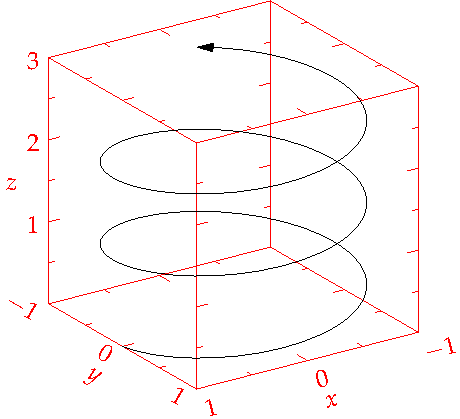
\includegraphics[width=\linewidth]{helix}
  \caption{This is a margin figure.  The helix is defined by 
    $x = \cos(2\pi z)$, $y = \sin(2\pi z)$, and $z = [0, 2.7]$.  The figure was
    drawn using Asymptote (\url{http://asymptote.sf.net/}).}
  \label{fig:marginfig}
\end{marginfigure}

\begin{docspec}
\textbackslash begin\{marginfigure\}\\
  \qquad\textbackslash includegraphics\{helix\}\\
  \qquad\textbackslash caption\{This is a margin figure.\}\\
  \qquad\textbackslash label\{fig:marginfig\}\\
\textbackslash end\{marginfigure\}\\
\end{docspec}

The \docenv{marginfigure} and \docenv{margintable} environments accept an optional parameter \docopt{offset} that adjusts the vertical position of the figure or table.  See the ``\nameref{sec:sidenotes}'' section above for examples.  The specifications are:
\begin{docspec}
  \textbackslash{begin\{marginfigure\}[\docopt{offset}]}\\
  \qquad\ldots\\
  \textbackslash{end\{marginfigure\}}\\
  \mbox{}\\
  \textbackslash{begin\{margintable\}[\docopt{offset}]}\\
  \qquad\ldots\\
  \textbackslash{end\{margintable\}}\\
\end{docspec}

Figure~\ref{fig:fullfig} is an example of the \docenv{figure*}
environment and figure~\ref{fig:textfig} is an example of the normal
\docenv{figure} environment.

\begin{figure*}[h]
  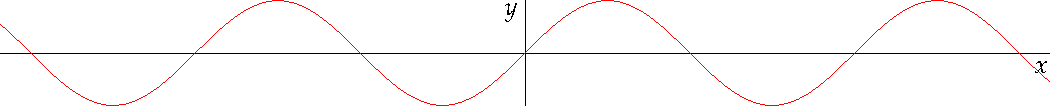
\includegraphics[width=\linewidth]{sine.pdf}%
  \caption{This graph shows $y = \sin x$ from about $x = [-10, 10]$.
  \emph{Notice that this figure takes up the full page width.}}%
  \label{fig:fullfig}%
\end{figure*}

\begin{figure}
  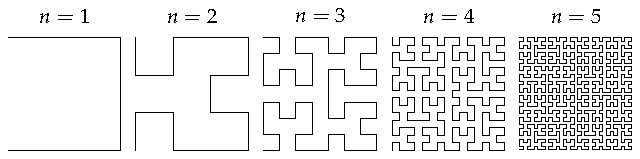
\includegraphics{hilbertcurves.pdf}
%  \checkparity This is an \pageparity\ page.%
  \caption[Hilbert curves of various degrees $n$.][6pt]{Hilbert curves of various degrees $n$. \emph{Notice that this figure only takes up the main textblock width.}}
  \label{fig:textfig}
  %\zsavepos{pos:textfig}
\end{figure}

\chapter{Conclusion}


%%
% The back matter contains appendices, bibliographies, indices, glossaries, etc.







\backmatter

\bibliography{biblio}
\bibliographystyle{apalike}


\printindex

\end{document}

